\documentclass[10pt,a4paper]{article}
\usepackage[utf8]{inputenc}
\usepackage[T1]{fontenc}
\usepackage[romanian]{babel}
\usepackage[margin=1.7cm]{geometry}
\usepackage{amsmath,amssymb,mathtools}
\usepackage{enumitem}
\usepackage{titlesec}
\usepackage{parskip}
\usepackage{tikz}
\usetikzlibrary{calc,arrows.meta,positioning}
\usepackage{pgfplots}
\pgfplotsset{compat=1.18}
\usepackage[most]{tcolorbox}
\usepackage{xcolor}

\newtcolorbox{res}{colback=red!6,colframe=red!65!black,boxrule=0.6pt,arc=1.5pt,
  left=4pt,right=4pt,top=2pt,bottom=2pt,breakable}
\newtcolorbox{chk}{colback=green!6,colframe=green!45!black,boxrule=0.6pt,arc=1.5pt,
  left=4pt,right=4pt,top=2pt,bottom=2pt,breakable}

\setlist{nosep, topsep=2pt, itemsep=2pt, leftmargin=1.3em}
\titlespacing*{\section}{0pt}{6pt}{2pt}
\titlespacing*{\subsection}{0pt}{4pt}{1pt}
\renewcommand{\baselinestretch}{0.96}
\setlength{\parindent}{0pt}
\pagestyle{empty}

\begin{document}
\begin{center}
{\large\bfseries Rezolvare --- Bilet de examen SAE}
\end{center}
\vspace{-0.2cm}

\section*{1. $G(s)=\dfrac{1}{s(s+5)}$, $T_e=0.1$s}

\subsection*{a) $H(z)$ -- metoda trapezului (Tustin)}
$$\textcolor{blue}{s=\frac2{T_e}\cdot\frac{z-1}{z+1}=20\,\frac{z-1}{z+1}}\qquad s+5=\frac{20(z-1)+5(z+1)}{z+1}=\frac{25z-15}{z+1}$$
$$G(z)=\frac1{s(s+5)}=\frac{(z+1)^2}{20(z-1)(25z-15)}=\frac{(z+1)^2}{100(z-1)(5z-3)}=\frac{z^2+2z+1}{500z^2-800z+300}$$
$$H(z)=\frac{G(z)}{1+G(z)}=\frac{z^2+2z+1}{(500z^2-800z+300)+(z^2+2z+1)}$$
\begin{res}
$$H(z)=\frac{z^2+2z+1}{501z^2-798z+301}$$
\end{res}

\subsection*{a2) $H(z)$ -- metoda matched (alternativă)}
$$\color{blue}p_d=e^{-p_cT_e},\quad z_d=e^{-z_cT_e}\qquad\text{(pas 1: poli \& zerouri)}$$
$$\color{blue}\text{dacă }n>m:\text{ se adaugă }(n-1)\text{ factori }(z+1)\text{ la numărător}\qquad\text{(pas 2)}$$
$$\color{blue}\lim_{s\to0}s^\sigma G(s)=\lim_{z\to1}\Big(\frac{z-1}{zT_e}\Big)^{\!\sigma}G(z)\qquad\text{(pas 3: câștigul }K_d\text{, }\sigma=\text{tipul sistemului)}$$
Poli $G(s)$: $s=0\to z=1$; $s=-5\to z=e^{-5\cdot0.1}=e^{-0.5}=0.6065$. Fără zerouri finite ($m=0$), $n=2\Rightarrow(n-1)=1$ factor $(z+1)$ adăugat:
$$G(z)=\frac{K_d(z+1)}{(z-1)(z-0.6065)}$$
Sistem tip 1 ($\sigma=1$):
$$\lim_{s\to0}sG(s)=\lim_{s\to0}\frac1{s+5}=\frac15\qquad
\lim_{z\to1}\frac{z-1}{zT_e}\cdot\frac{K_d(z+1)}{(z-1)(z-0.6065)}=\frac{2K_d}{T_e(1-0.6065)}$$
$$\frac15=\frac{2K_d}{0.1\cdot0.3935}\ \Rightarrow\ K_d=0.0039$$
\begin{res}
$$G(z)=\frac{0.0039(z+1)}{(z-1)(z-0.6065)}=\frac{0.0039z+0.0039}{z^2-1.6065z+0.6065}$$
$$H(z)=\frac{G(z)}{1+G(z)}=\frac{0.0039z+0.0039}{z^2-1.6026z+0.6105}$$
\end{res}
(comparativ cu Tustin: aceiași pași b)/c) se aplică identic, doar cu polii/coeficienții de mai sus.)

\subsection*{b) Eroare staționară}
$$G(z)=\frac{(z+1)^2}{100(z-1)(5z-3)}$$
$$K_p=\lim_{z\to1}G(z)=\infty\qquad
K_v=\frac1{T_e}\lim_{z\to1}(z-1)G(z)=\frac1{0.1}\cdot\frac{4}{100\cdot2}=10\cdot0.02=0.2$$
$$K_a=\frac1{T_e^2}\lim_{z\to1}(z-1)^2G(z)=\lim_{z\to1}(z-1)\cdot\frac{(z+1)^2}{T_e\cdot100(5z-3)}=0$$
\begin{res}
$$e_{ss}(\text{treaptă})=\frac1{1+K_p}=0\qquad
e_{ss}(\text{rampă})=\frac1{K_v}=\frac1{0.2}=5\qquad
e_{ss}(\text{parabolă})=\frac1{K_a}=\infty$$
\end{res}

\subsection*{c) Răspuns la impuls unitar Dirac ($\mathcal Z^{-1}$)}
$$Y(z)=H(z)\cdot R(z)=H(z)=\frac{z^2+2z+1}{501z^2-798z+301}$$
$$z_{1,2}=\frac{798\pm\sqrt{798^2-4\cdot501\cdot301}}{2\cdot501}\ \Rightarrow\ z_1=0.9793,\quad z_2=0.6135$$
$$\frac{Y(z)}z=\frac{C_0}z+\frac{C_1}{z-z_1}+\frac{C_2}{z-z_2}\qquad
\textcolor{blue}{\mathcal Z^{-1}\Big\{\frac zz\Big\}=\delta(k),\qquad \mathcal Z^{-1}\Big\{\frac{z}{z-a}\Big\}=a^k}$$
$$C_0=\frac1{301}=0.0033\qquad C_1=\frac{(z_1+1)^2}{501\,z_1(z_1-z_2)}=0.0218\qquad C_2=\frac{(z_2+1)^2}{501\,z_2(z_2-z_1)}=-0.0232$$
\begin{res}
$$y(k)=0.0033\,\delta(k)+0.0218\,(0.9793)^k-0.0232\,(0.6135)^k,\qquad k\ge0$$
\end{res}
\begin{center}
\begin{tabular}{@{}rrrrrrrrrr@{}}
$k$&0&1&2&3&4&5&6&7&8\\
$y(k)$&0.0020&0.0072&0.0122&0.0152&0.0168&0.0176&0.0180&0.0181&0.0180\\
\end{tabular}
\end{center}

\begin{center}
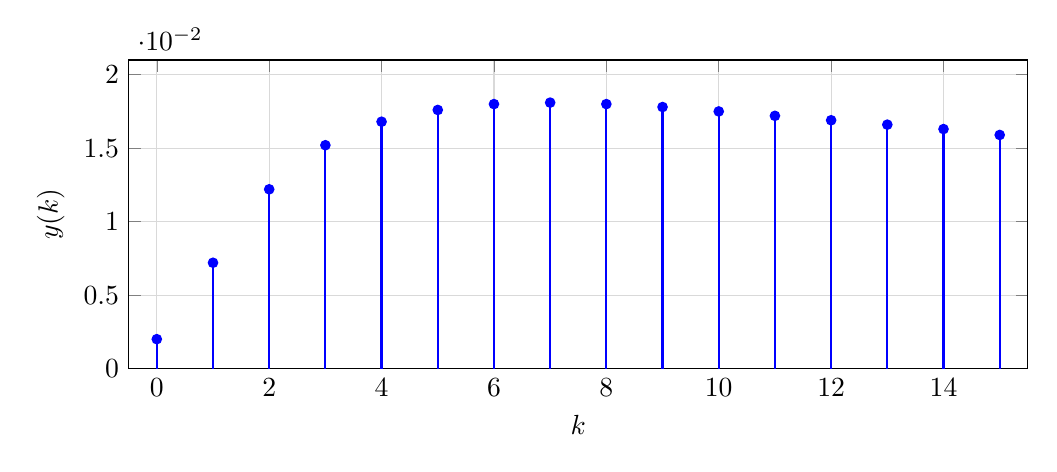
\begin{tikzpicture}
\begin{axis}[
  width=13cm,height=5.5cm,
  xlabel={$k$}, ylabel={$y(k)$},
  xmin=-0.5,xmax=15.5, ymin=0, ymax=0.0210,
  grid=both, minor grid style={gray!15}, major grid style={gray!30},
]
\addplot[ycomb,thick,blue,mark=*,mark size=1.5pt,mark options={fill=blue}] coordinates {
(0,0.0020) (1,0.0072) (2,0.0122) (3,0.0152) (4,0.0168) (5,0.0176) (6,0.0180) (7,0.0181)
(8,0.0180) (9,0.0178) (10,0.0175) (11,0.0172) (12,0.0169) (13,0.0166) (14,0.0163) (15,0.0159)
};
\end{axis}
\end{tikzpicture}
\end{center}

\section*{2. $G_d(z)=\dfrac{0.2z+0.07}{z^2-0.5z+0.05}$, $T_e=1$s (circuit deschis)}
$$\color{blue}z=\frac{1+\frac{T_e}2w}{1-\frac{T_e}2w}\overset{T_e=1}{=}\frac{1+0.5w}{1-0.5w}=\frac ND,\ N=1{+}0.5w,\ D=1{-}0.5w$$
$$0.2z+0.07=\frac{0.2N+0.07D}D=\frac{0.27+0.07w}D$$
$$z^2-0.5z+0.05=\frac{N^2-0.5ND+0.05D^2}{D^2}=\frac{0.39w^2+0.95w+0.55}{D^2}$$
\begin{res}
$$G_d(w)=\frac{(0.27+0.07w)\,D}{0.39w^2+0.95w+0.55}=\frac{-0.03w^2-0.07w+0.27}{0.39w^2+0.95w+0.55}$$
\end{res}
$$N(w)=0\Rightarrow w_{z1}=2,\quad w_{z2}=-4.15\qquad D(w)=0\Rightarrow w_{p1}=-0.94,\quad w_{p2}=-1.51$$
\begin{res}
$$G_d(w)=\underbrace{\frac{0.27}{0.55}}_{K_B=0.49}\cdot\frac{\left(1-\dfrac w2\right)\left(1+\dfrac w{4.15}\right)}{\left(1+\dfrac w{0.94}\right)\left(1+\dfrac w{1.51}\right)}$$
\end{res}
$w_{z1}=2>0\Rightarrow$ zerou neminim-fazic.
Frecvențe de frângere (rad/s): $\omega_{p1}=0.94,\ \omega_{p2}=1.51,\ \omega_{z1}=2,\ \omega_{z2}=4.15$.
\begin{res}
Panta asimptotică a modulului (nivel de start $20\lg K_B=-6.18$dB):
$$\underbrace{0}_{\omega<0.94}\to\underbrace{-20}_{0.94<\omega<1.51}\to\underbrace{-40}_{1.51<\omega<2}\to\underbrace{-20}_{2<\omega<4.15}\to\underbrace{0}_{\omega>4.15}\ \text{dB/dec}$$
Nivel final ($\omega\to\infty$): $20\lg\left|\dfrac{-0.03}{0.39}\right|=-21.53$dB (raport coeficienți dominanți).
Fază asimptotică ($\omega\to\infty$): $2\text{ poli}(-90^\circ)+1\text{ zerou m.f.}(+90^\circ)+1\text{ zerou n.m.f.}(-90^\circ)=-180^\circ$.
\end{res}
\begin{res}
\begin{center}
\begin{tabular}{@{}rrrrrrrrrr@{}}
$\omega$&0.01&0.1&0.5&1&2&5&10&50&100\\
$|G_d|_{dB}$&$-6.18$&$-6.24$&$-7.39$&$-9.84$&$-14.09$&$-19.14$&$-20.80$&$-21.50$&$-21.52$\\
$\varphi\,[^\circ]$&$-1.1$&$-11.4$&$-53.5$&$-93.3$&$-137.0$&$-170.5$&$-177.3$&$-179.7$&$-179.8$\\
\end{tabular}
\end{center}
\end{res}

\begin{center}
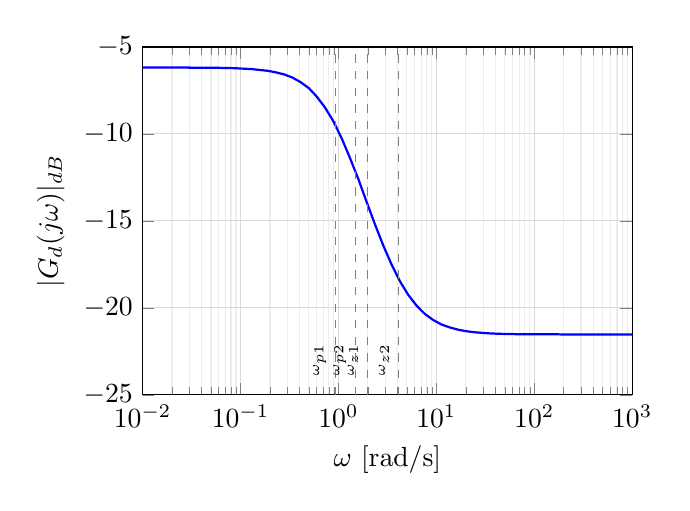
\begin{tikzpicture}
\begin{semilogxaxis}[
  width=7.8cm,height=6cm,
  xlabel={$\omega$ [rad/s]}, ylabel={$|G_d(j\omega)|_{dB}$},
  xmin=0.01,xmax=1000, ymin=-25,ymax=-5,
  grid=both, minor grid style={gray!15}, major grid style={gray!30},
]
\addplot[blue,thick] coordinates {
(0.01,-6.18) (0.01,-6.18) (0.01,-6.18) (0.02,-6.18) (0.02,-6.18) (0.03,-6.18) (0.03,-6.19) (0.04,-6.19) (0.05,-6.19) (0.06,-6.20) (0.07,-6.21) (0.09,-6.22) (0.10,-6.24) (0.13,-6.27) (0.15,-6.31) (0.19,-6.37) (0.23,-6.46) (0.28,-6.58) (0.34,-6.76) (0.41,-7.02) (0.50,-7.37) (0.60,-7.85) (0.73,-8.48) (0.89,-9.28) (1.08,-10.25) (1.31,-11.37) (1.60,-12.60) (1.94,-13.90) (2.36,-15.19) (2.87,-16.41) (3.49,-17.51) (4.24,-18.46) (5.15,-19.24) (6.26,-19.86) (7.61,-20.34) (9.25,-20.69) (11.24,-20.95) (13.66,-21.12) (16.61,-21.25) (20.19,-21.34) (24.54,-21.40) (29.82,-21.44) (36.25,-21.47) (44.06,-21.49) (53.56,-21.50) (65.10,-21.51) (79.12,-21.52) (96.17,-21.52) (116.9,-21.52) (142.08,-21.52) (172.7,-21.52) (209.91,-21.53) (255.14,-21.53) (310.12,-21.53) (376.94,-21.53) (458.16,-21.53) (556.88,-21.53) (676.88,-21.53) (822.72,-21.53) (1000,-21.53)
};
\addplot[gray,dashed] coordinates {(0.94,-25)(0.94,-5)};
\addplot[gray,dashed] coordinates {(1.51,-25)(1.51,-5)};
\addplot[gray,dashed] coordinates {(2,-25)(2,-5)};
\addplot[gray,dashed] coordinates {(4.15,-25)(4.15,-5)};
\node[above,rotate=90,font=\tiny] at (axis cs:0.94,-23) {$\omega_{p1}$};
\node[above,rotate=90,font=\tiny] at (axis cs:1.51,-23) {$\omega_{p2}$};
\node[above,rotate=90,font=\tiny] at (axis cs:2,-23) {$\omega_{z1}$};
\node[above,rotate=90,font=\tiny] at (axis cs:4.15,-23) {$\omega_{z2}$};
\end{semilogxaxis}
\end{tikzpicture}
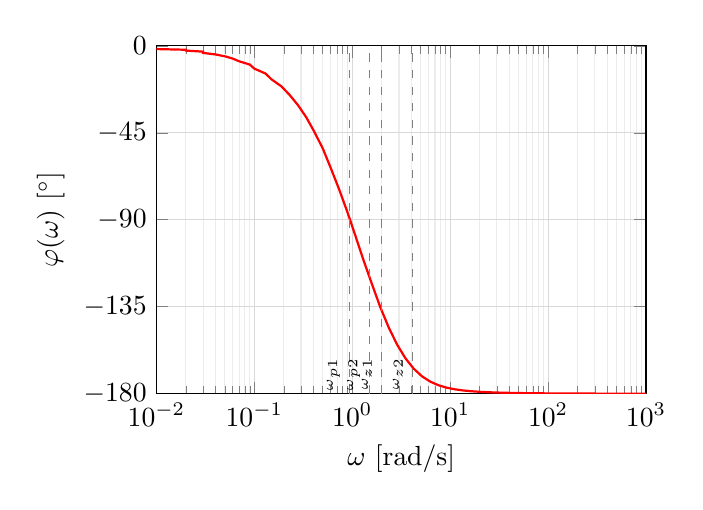
\begin{tikzpicture}
\begin{semilogxaxis}[
  width=7.8cm,height=6cm,
  xlabel={$\omega$ [rad/s]}, ylabel={$\varphi(\omega)$ [$^\circ$]},
  xmin=0.01,xmax=1000, ymin=-180,ymax=0,
  ytick={-180,-135,-90,-45,0},
  grid=both, minor grid style={gray!15}, major grid style={gray!30},
]
\addplot[red,thick] coordinates {
(0.01,-1.14) (0.01,-1.38) (0.01,-1.68) (0.02,-2.04) (0.02,-2.48) (0.03,-3.02) (0.03,-3.67) (0.04,-4.46) (0.05,-5.42) (0.06,-6.58) (0.07,-8.00) (0.09,-9.72) (0.10,-11.80) (0.13,-14.32) (0.15,-17.37) (0.19,-21.06) (0.23,-25.48) (0.28,-30.78) (0.34,-37.07) (0.41,-44.48) (0.50,-53.08) (0.60,-62.91) (0.73,-73.88) (0.89,-85.82) (1.08,-98.41) (1.31,-111.21) (1.60,-123.70) (1.94,-135.38) (2.36,-145.77) (2.87,-154.56) (3.49,-161.63) (4.24,-167.03) (5.15,-170.97) (6.26,-173.74) (7.61,-175.63) (9.25,-176.90) (11.24,-177.75) (13.66,-178.33) (16.61,-178.74) (20.19,-179.02) (24.54,-179.23) (29.82,-179.39) (36.25,-179.51) (44.06,-179.60) (53.56,-179.67) (65.10,-179.73) (79.12,-179.78) (96.17,-179.82) (116.9,-179.85) (142.08,-179.88) (172.7,-179.90) (209.91,-179.92) (255.14,-179.93) (310.12,-179.94) (376.94,-179.96) (458.16,-179.96) (556.88,-179.97) (676.88,-179.97) (822.72,-179.98) (1000,-179.98)
};
\addplot[gray,dashed] coordinates {(0.94,-180)(0.94,0)};
\addplot[gray,dashed] coordinates {(1.51,-180)(1.51,0)};
\addplot[gray,dashed] coordinates {(2,-180)(2,0)};
\addplot[gray,dashed] coordinates {(4.15,-180)(4.15,0)};
\node[above,rotate=90,font=\tiny] at (axis cs:0.94,-170) {$\omega_{p1}$};
\node[above,rotate=90,font=\tiny] at (axis cs:1.51,-170) {$\omega_{p2}$};
\node[above,rotate=90,font=\tiny] at (axis cs:2,-170) {$\omega_{z1}$};
\node[above,rotate=90,font=\tiny] at (axis cs:4.15,-170) {$\omega_{z2}$};
\end{semilogxaxis}
\end{tikzpicture}
\end{center}

\section*{3. $G_d(z)=\dfrac{k(0.13z+0.02)}{z^2-0.39z+0.007}$, $T_e=1$s}
$$z^2-0.39z+0.007=0\ \Rightarrow\ p_1=0.37,\ p_2=0.02\qquad 0.13z+0.02=0\ \Rightarrow\ z_0=-0.15$$

\subsection*{a) Ramuri}
$n=2$, $m=1\Rightarrow$ nr. ramuri $=2$.
\begin{res}
Ramuri din $p_1=0.37$, $p_2=0.02$; se termină în $z_0=-0.15$ și în $z\to\infty$.
\end{res}

\subsection*{b) Axa reală}
\begin{res}
$$(p_2,\,p_1)=(0.02,\,0.37)\qquad(-\infty,\,z_0)=(-\infty,\,-0.15)$$
\end{res}

\subsection*{c) Asimptote}
$$n-m=1,\qquad \textcolor{blue}{\theta=\frac{180^\circ(2i+1)}{n-m}}\Big|_{i=0}=180^\circ\qquad
\textcolor{blue}{\sigma_a=\frac{\sum p_i-\sum z_i}{n-m}}=\frac{0.39-(-0.15)}1=0.54$$
\begin{res}
1 asimptotă, $180^\circ$, $\sigma_a=0.54$.
\end{res}

\subsection*{d) Puncte de ramificație}
$$\color{blue}1+G_d(z)=0\Rightarrow k(z)=-\dfrac{N(z)}{D(z)}$$
$$N(z)=z^2-0.39z+0.007,\qquad D(z)=0.13z+0.02$$
$$\textcolor{blue}{\frac{dk}{dz}=0\ \Leftrightarrow\ N'(z)D(z)-N(z)D'(z)=0,}\qquad N'=2z-0.39,\ D'=0.13$$
$$(2z-0.39)(0.13z+0.02)-0.13(z^2-0.39z+0.007)=0$$
\begin{res}
$$0.13z^2+0.04z-0.01=0$$
\end{res}
$$z=\frac{-0.04\pm\sqrt{0.04^2+4\cdot0.13\cdot0.01}}{2\cdot0.13}$$
\begin{res}
$$z_{b1}=0.15\ (k\approx0.73)\qquad z_{b2}=-0.45\ (k\approx10.00)$$
\end{res}

\subsection*{e) Cerc \& trasare}
$$\color{blue}z=z_0+w,\quad |w|^2=(z_0-p_1)(z_0-p_2)$$
$$\color{blue}r=|w|=\sqrt{(z_0-p_1)(z_0-p_2)}$$
$$z_0-p_1=-0.52\qquad z_0-p_2=-0.17\qquad r=\sqrt{0.09}$$
\begin{res}
$$r=0.30$$
\end{res}
$|z_{b1}-z_0|=|0.15-(-0.15)|=0.30$; $|z_{b2}-z_0|=|-0.45-(-0.15)|=0.30$ $\checkmark$

\begin{center}
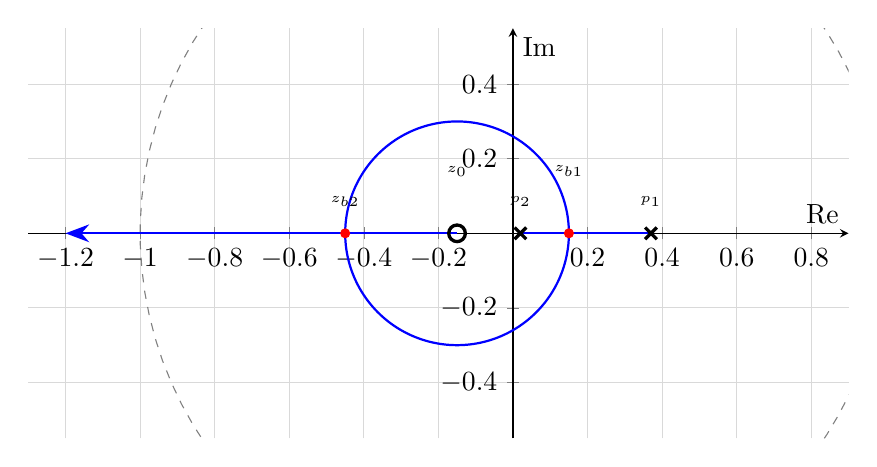
\begin{tikzpicture}
\begin{axis}[
  width=12cm,height=8cm,
  xlabel={$\mathrm{Re}$}, ylabel={$\mathrm{Im}$},
  xmin=-1.3,xmax=0.9,ymin=-0.55,ymax=0.55,
  axis equal image,
  axis lines=middle,
  grid=both, minor grid style={gray!15}, major grid style={gray!30},
]
\addplot[gray,dashed,domain=0:360,samples=100] ({cos(x)},{sin(x)});
\addplot[blue,thick,domain=0:360,samples=200] ({-0.15+0.30*cos(x)},{0.30*sin(x)});
\addplot[blue,thick] coordinates {(0.02,0)(0.15,0)};
\addplot[blue,thick] coordinates {(0.15,0)(0.37,0)};
\addplot[blue,thick] coordinates {(-0.45,0)(-0.15,0)};
\addplot[blue,thick,-{Stealth[length=3mm]}] coordinates {(-0.45,0)(-1.2,0)};
\addplot[only marks,mark=x,black,mark size=3pt,line width=1.2pt] coordinates {(0.37,0)(0.02,0)};
\addplot[only marks,mark=o,black,mark size=3pt,line width=1.2pt] coordinates {(-0.15,0)};
\addplot[only marks,mark=*,red,mark size=1.6pt] coordinates {(0.15,0)(-0.45,0)};
\node[above,yshift=6pt] at (axis cs:-0.45,0) {\tiny $z_{b2}$};
\node[above,yshift=17pt] at (axis cs:-0.15,0) {\tiny $z_0$};
\node[above,yshift=6pt] at (axis cs:0.02,0) {\tiny $p_2$};
\node[above,yshift=17pt] at (axis cs:0.15,0) {\tiny $z_{b1}$};
\node[above,yshift=6pt] at (axis cs:0.37,0) {\tiny $p_1$};
\end{axis}
\end{tikzpicture}
\end{center}
(cerc punctat = cerc unitate.)

\subsection*{f) Curbă polară ($k=1$)}
$$\color{blue}z=\frac{1+\frac{T_e}2w}{1-\frac{T_e}2w}\overset{T_e=1}{=}\frac{1+0.5w}{1-0.5w}=\frac ND,\quad N=1+0.5w,\ D=1-0.5w$$
Se înlocuiește $z=N/D$ în $G_d(z)$ (ca la Bode) și se amplifică cu $D^2$:
$$G_d(w)=\frac{(0.13N+0.02D)D}{N^2-0.39ND+0.007D^2}=\frac{-0.0275w^2-0.02w+0.15}{0.34925w^2+0.993w+0.617}$$
$$\color{blue}w=j\omega\ \Rightarrow\ G_d(j\omega)=\mathrm{Re}(\omega)+j\,\mathrm{Im}(\omega),\qquad \omega\in[0,\infty)$$
Capetele curbei: $\omega=0$ ($z=1$); $\omega\to\infty$ ($z=-1$).
\begin{res}
$$G_d(j0)=\frac{0.15}{0.617}=0.2431\ (\text{start})\qquad \lim_{\omega\to\infty}G_d(j\omega)=\frac{-0.0275}{0.34925}=-0.0787\ (\text{final})$$
\end{res}
\begin{res}
\begin{center}
\begin{tabular}{@{}rrrrrrrrrr@{}}
$\omega$&0&0.2&0.5&1&2&3&5&10&30\\
$\mathrm{Re}$&0.2431&0.2241&0.1482&0.0262&$-0.0620$&$-0.0775$&$-0.0806$&$-0.0796$&$-0.0788$\\
$\mathrm{Im}$&0&$-0.0804$&$-0.1578$&$-0.1717$&$-0.1066$&$-0.0677$&$-0.0370$&$-0.0172$&$-0.0056$\\
\end{tabular}
\end{center}
\end{res}
\begin{center}
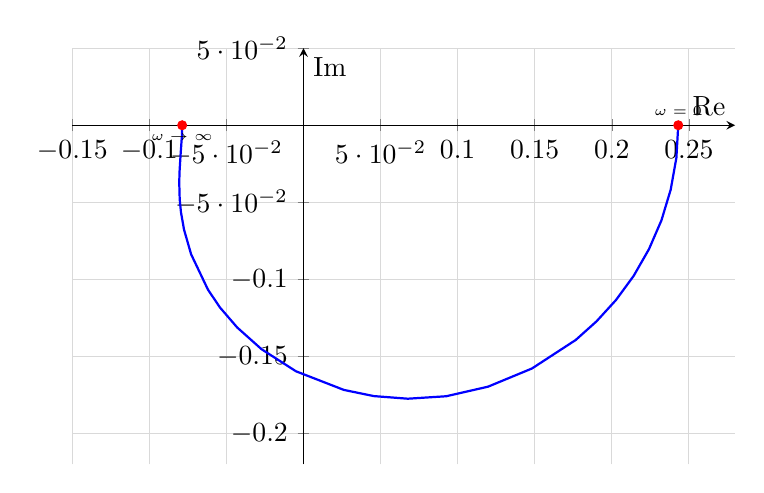
\begin{tikzpicture}
\begin{axis}[
  width=10cm,height=8cm,
  xlabel={$\mathrm{Re}$}, ylabel={$\mathrm{Im}$},
  xmin=-0.15,xmax=0.28,ymin=-0.22,ymax=0.05,
  axis equal image,
  axis lines=middle,
  grid=both, minor grid style={gray!15}, major grid style={gray!30},
]
\addplot[blue,thick,mark=none] coordinates {
(0.2431,0.0000) (0.2419,-0.0211) (0.2382,-0.0418) (0.2322,-0.0617) (0.2241,-0.0804) (0.2142,-0.0977) (0.2027,-0.1134) (0.1901,-0.1272) (0.1766,-0.1393) (0.1482,-0.1578) (0.1197,-0.1696) (0.0926,-0.1758) (0.0677,-0.1774) (0.0456,-0.1757) (0.0262,-0.1717) (-0.0049,-0.1596) (-0.0272,-0.1453) (-0.0430,-0.1312) (-0.0542,-0.1182) (-0.0620,-0.1066) (-0.0729,-0.0837) (-0.0775,-0.0677) (-0.0795,-0.0563) (-0.0803,-0.0481) (-0.0806,-0.0370) (-0.0804,-0.0300) (-0.0799,-0.0218) (-0.0796,-0.0172) (-0.0793,-0.0131) (-0.0791,-0.0099) (-0.0789,-0.0076) (-0.0788,-0.0056) (-0.0788,-0.0042) (-0.0788,-0.0030) (-0.0788,-0.0022) (-0.0787,-0.0017)
};
\addplot[only marks,mark=*,red,mark size=1.6pt] coordinates {(0.2431,0.0000) (-0.0787,-0.0000)};
\node[above] at (axis cs:0.2431,0.0000) {\tiny $\omega=0$};
\node[below] at (axis cs:-0.0787,0.0000) {\tiny $\omega\to\infty$};
\end{axis}
\end{tikzpicture}
\end{center}

\section*{4. $G_0(z)=\dfrac{0.02z+0.02}{z^2-1.49z+0.54}$}

\subsection*{a) Forma complet controlabilă}
$$\textcolor{blue}{G_0(z)=\frac{b_1z+b_0}{z^2+a_1z+a_0}},\quad a_1=-1.49,\ a_0=0.54,\ b_1=b_0=0.02$$
$$\color{blue}y(k{+}2)+a_1y(k{+}1)+a_0y(k)=b_1r(k{+}1)+b_0r(k)$$
$$\color{blue}x_1(k)=y(k),\quad x_2(k)=x_1(k{+}1)-b_0r(k)$$
$$\color{blue}x_1(k{+}1)=x_2(k)\qquad x_2(k{+}1)=-a_0x_1(k)-a_1x_2(k)+r(k)\qquad y(k)=b_0x_1(k)+b_1x_2(k)$$
\begin{res}
$$\Phi=\begin{pmatrix}0&1\\-0.54&1.49\end{pmatrix},\quad \Gamma=\begin{pmatrix}0\\1\end{pmatrix},\quad C=\begin{pmatrix}0.02&0.02\end{pmatrix},\quad D=0$$
\end{res}
\begin{chk}
$$zI-\Phi=\begin{pmatrix}z&-1\\0.54&z-1.49\end{pmatrix},\ \det=z^2-1.49z+0.54$$
$$C(zI-\Phi)^{-1}\Gamma=\frac{(0.02\ \ 0.02)\begin{pmatrix}1\\z\end{pmatrix}}{z^2-1.49z+0.54}=\frac{0.02z+0.02}{z^2-1.49z+0.54}=G_0(z)\ \checkmark$$
\end{chk}

\subsection*{b) Observabilitate}
$$\textcolor{blue}{Q=\begin{pmatrix}C\\C\Phi\end{pmatrix}},\qquad C\Phi=(0.02\ \ 0.02)\begin{pmatrix}0&1\\-0.54&1.49\end{pmatrix}=(-0.0108\ \ 0.0498)$$
\begin{res}
$$Q=\begin{pmatrix}0.02&0.02\\-0.0108&0.0498\end{pmatrix}\qquad \det Q=0.02\cdot0.0498-0.02\cdot(-0.0108)=0.0012\ne0$$
\end{res}
$\mathrm{rang}(Q)=2=n\Rightarrow$ \textbf{sistem complet observabil}.

\end{document}
